\begin{figure}[!hp]
    \centering
    \begin{tabular}{l c c c}
        \rotatebox{90}{\hspace{3em}MIMIC-IV} 
        &
        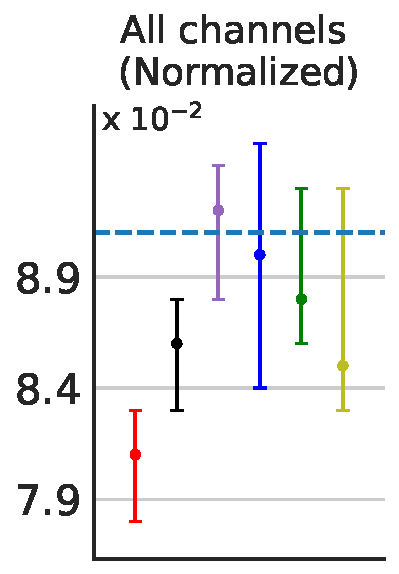
\includegraphics[height=5.2cm]{content/chapters/irregular_time_series_data_driven_missingness/figures/mimic_evaluation_summary.pdf} 
        &
        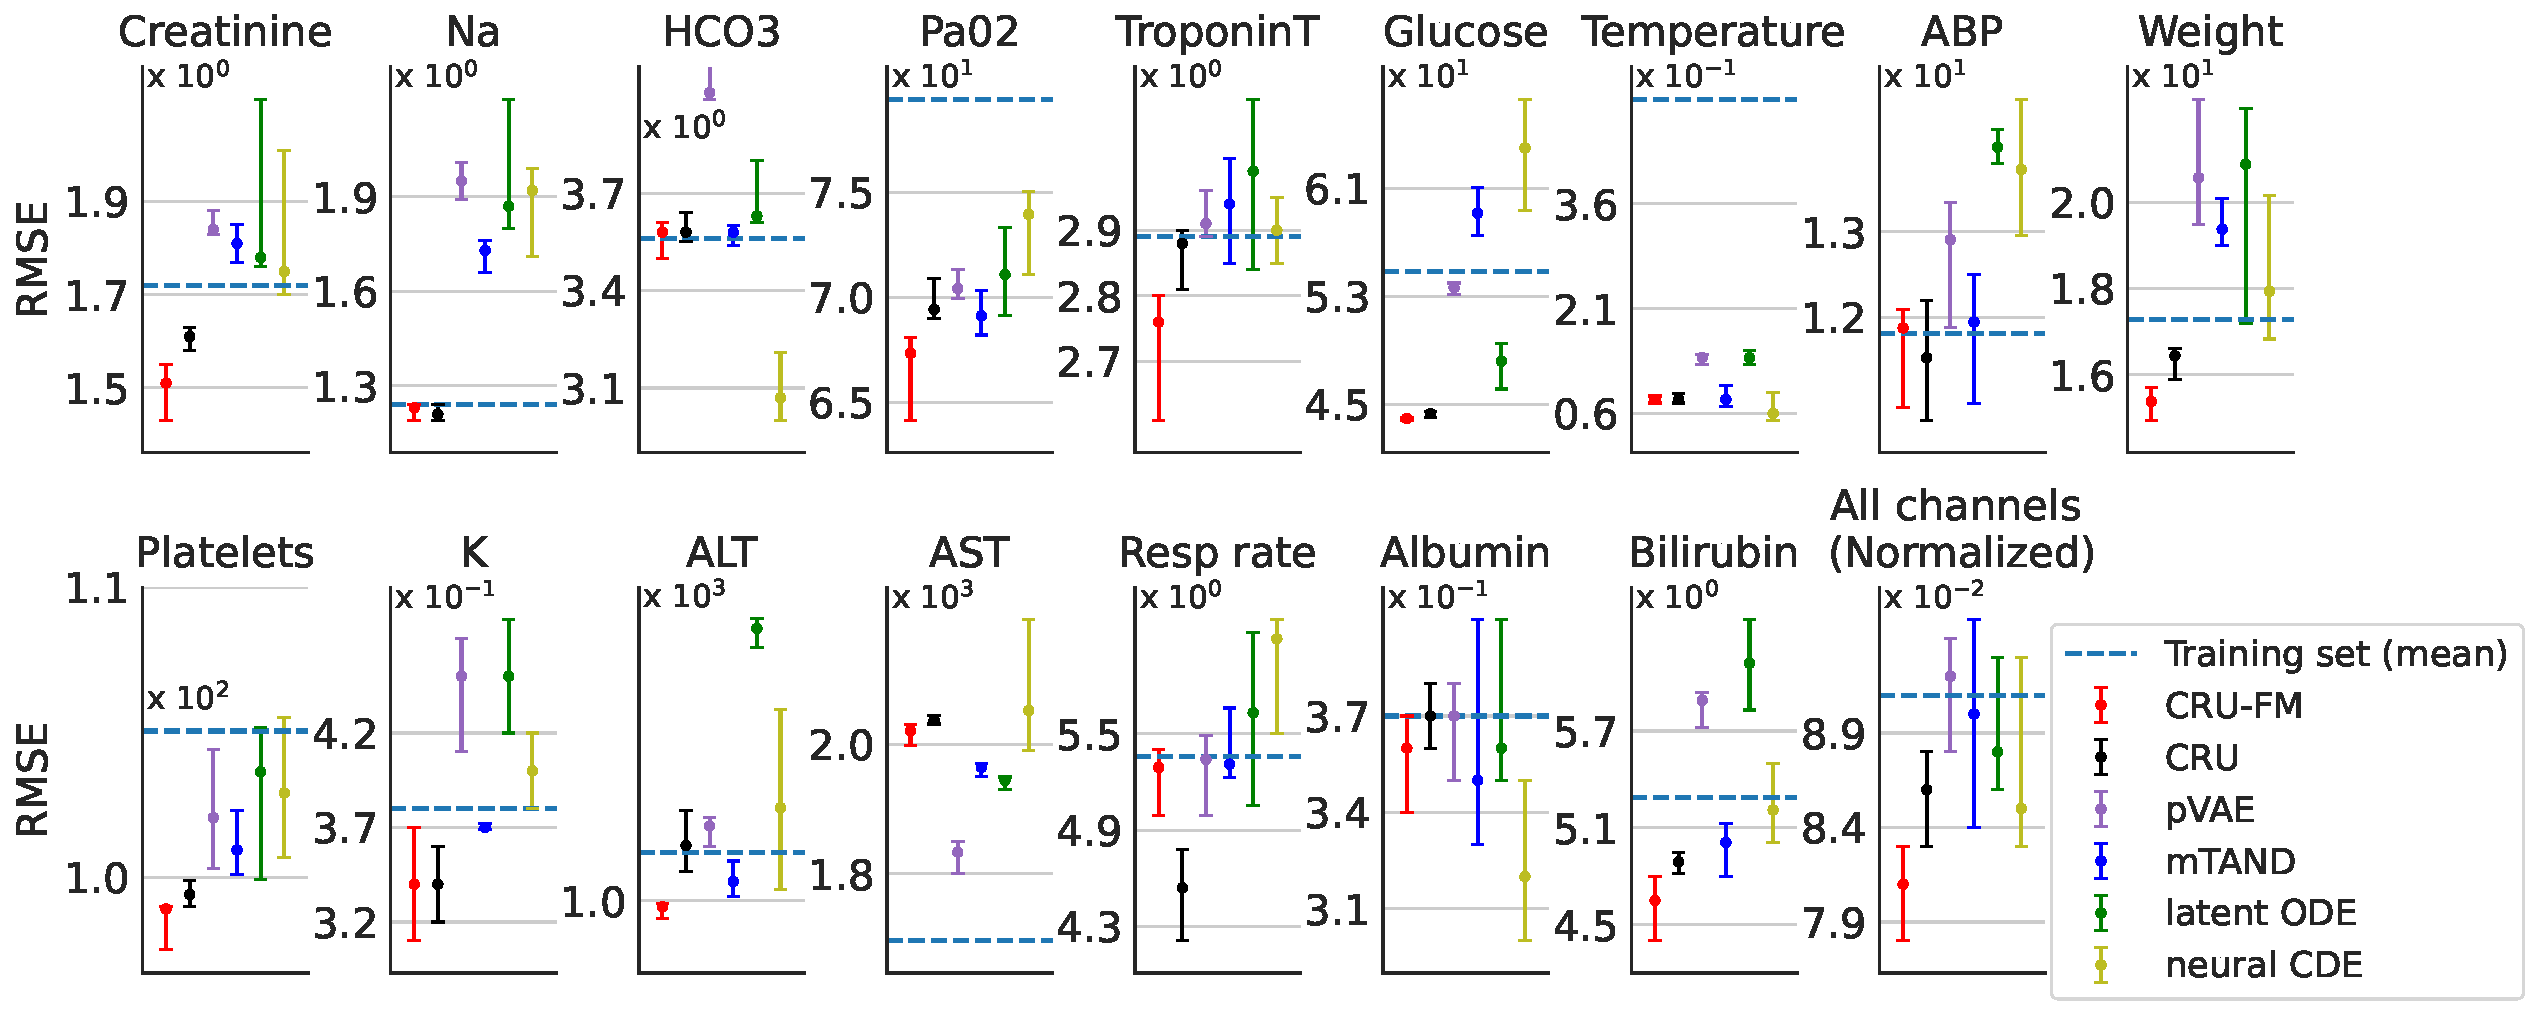
\includegraphics[trim={0 0 590 0},clip,height=5.2cm]{content/chapters/irregular_time_series_data_driven_missingness/figures/mimic_evaluation.pdf} 
        &
        \raisebox{1.5cm}{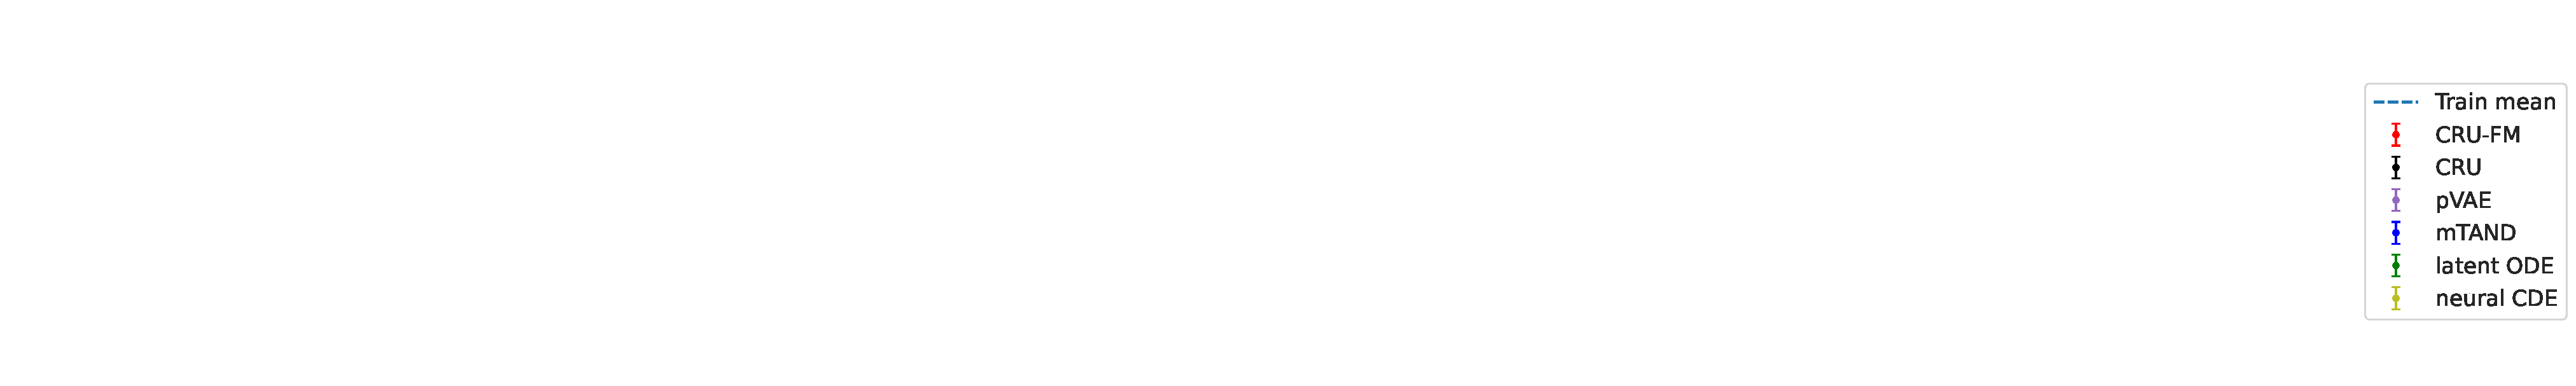
\includegraphics[height=3.5cm]{content/chapters/irregular_time_series_data_driven_missingness/figures/legend.pdf}}
    \\~\\
        \rotatebox{90}{\hspace{4em} Physionet} 
        & 
        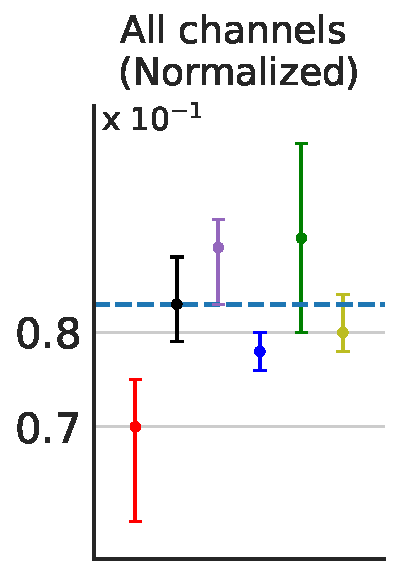
\includegraphics[height=5.2cm]{content/chapters/irregular_time_series_data_driven_missingness/figures/physionet_evaluation_summary.pdf} 
        &
        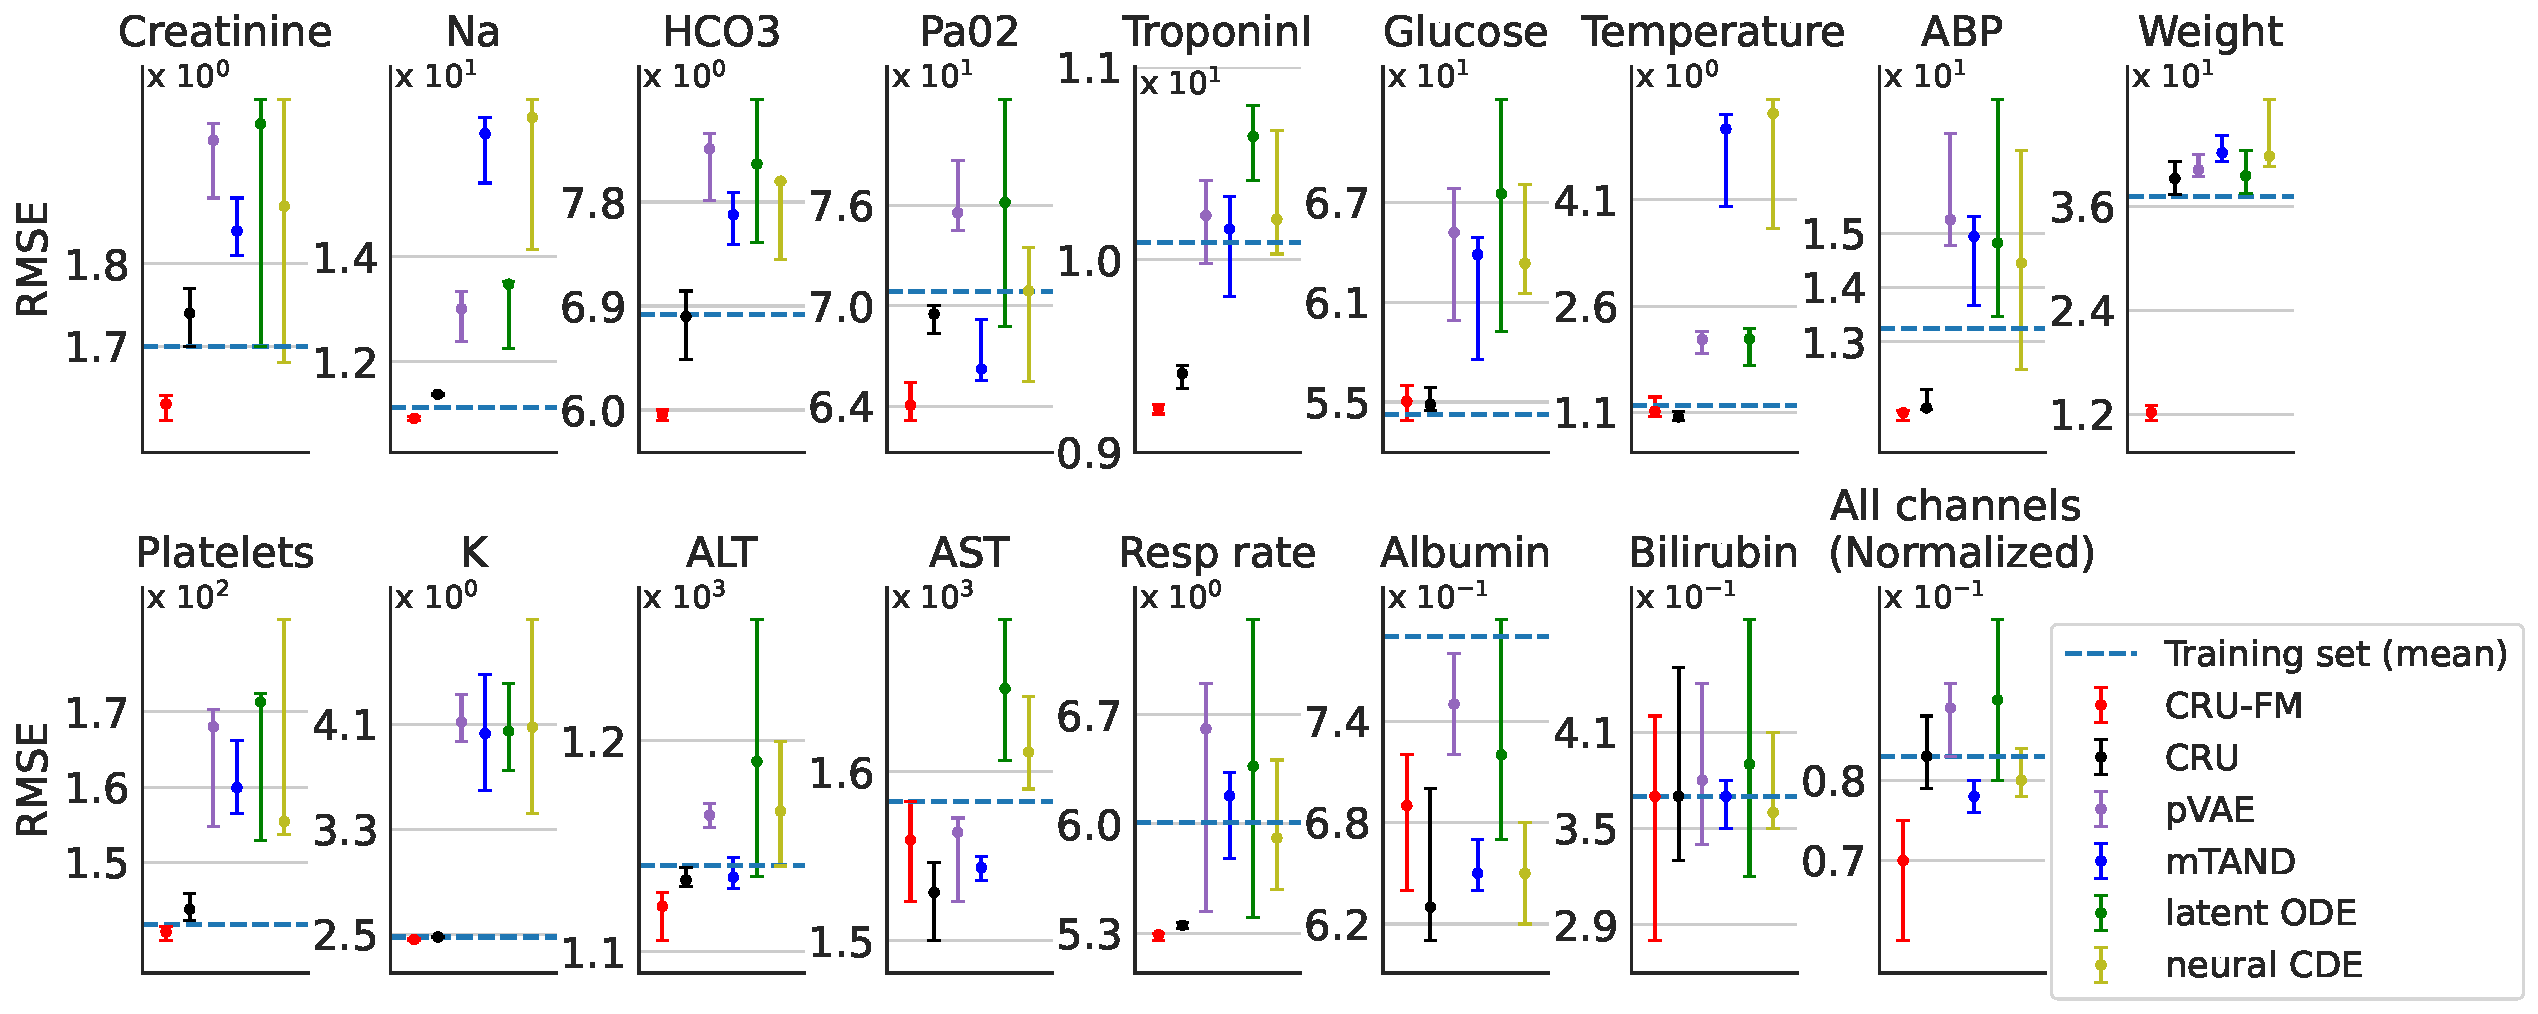
\includegraphics[trim={0 0 590 0},clip,height=5.2cm]{content/chapters/irregular_time_series_data_driven_missingness/figures/physionet_evaluation.pdf}
    \\~\\
        \rotatebox{90}{\hspace{4em} eICU}
        &
        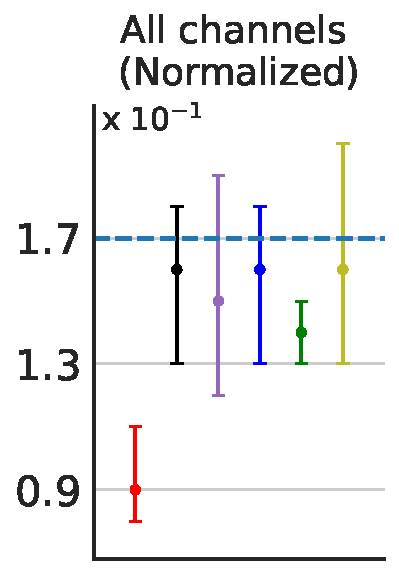
\includegraphics[height=5.2cm]{content/chapters/irregular_time_series_data_driven_missingness/figures/eicu_evaluation_summary.pdf} 
        &
        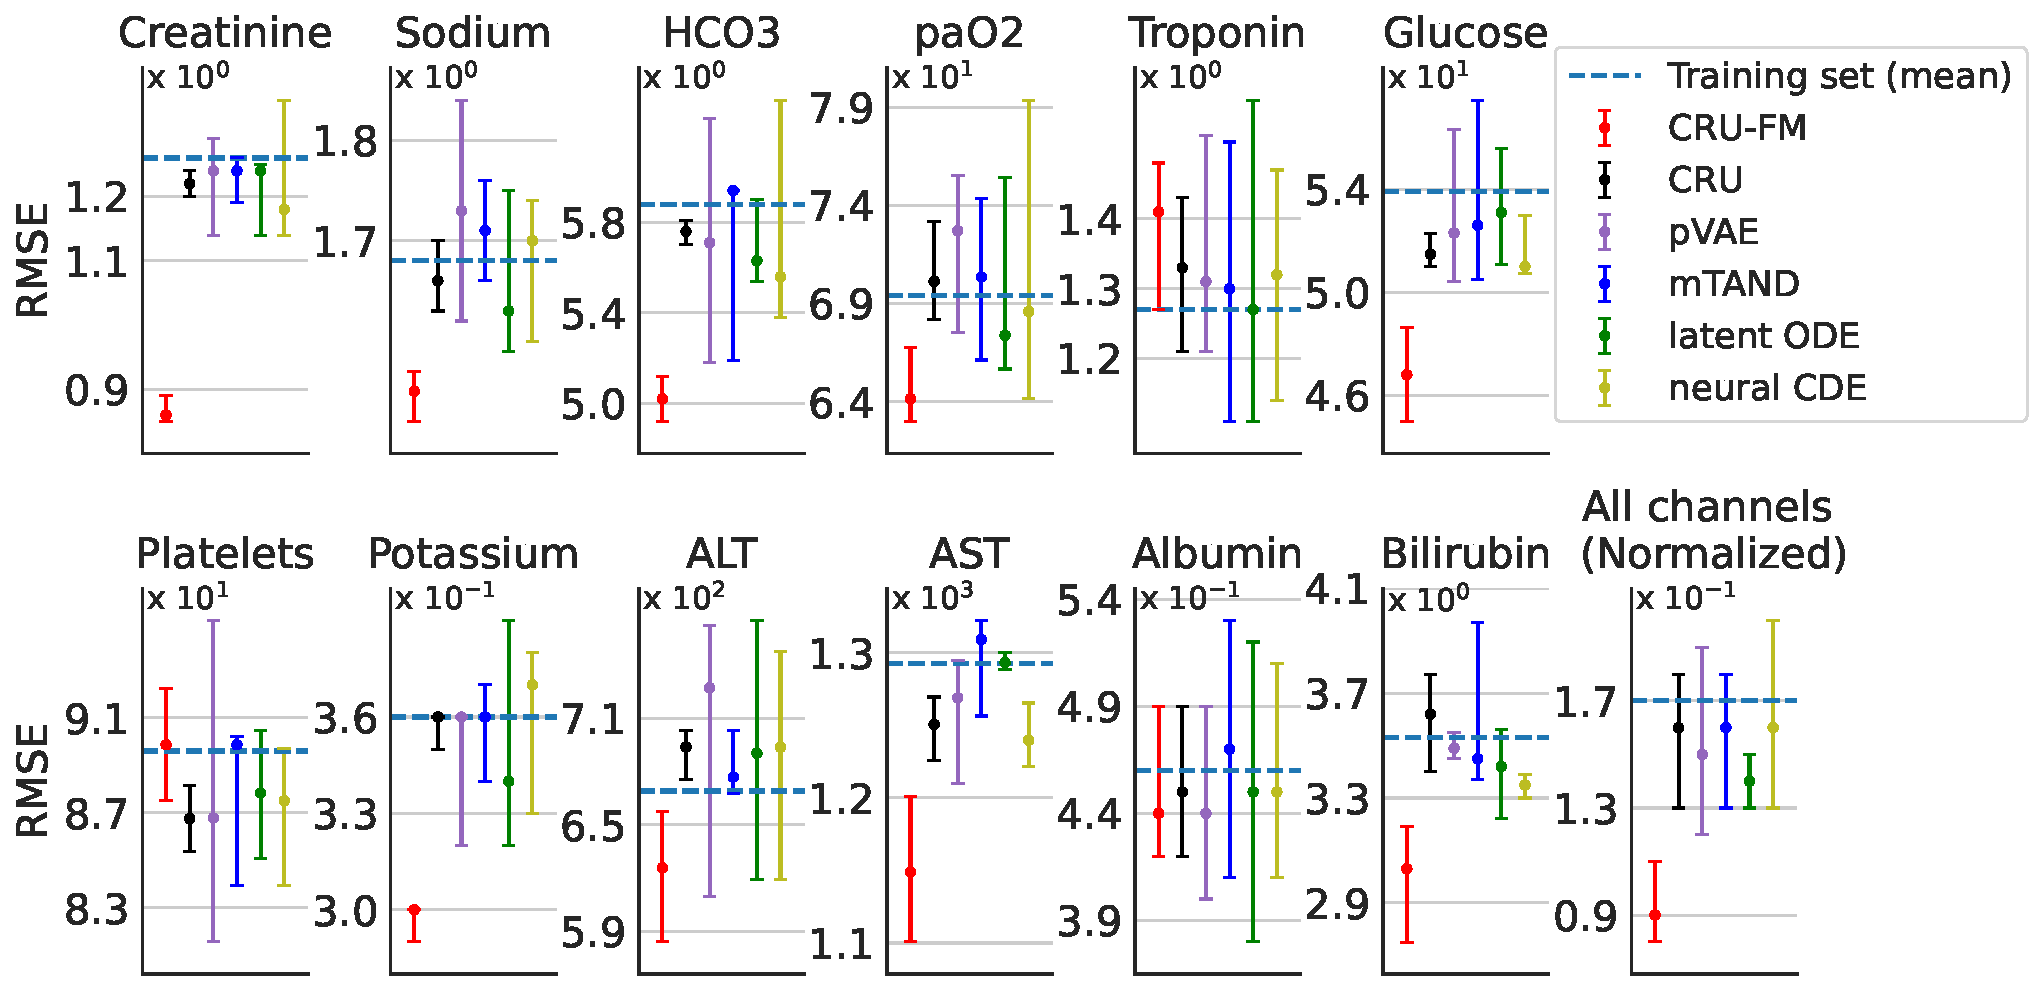
\includegraphics[trim={0 0 355 0},clip,height=5.2cm]{content/chapters/irregular_time_series_data_driven_missingness/figures/eicu_evaluation.pdf}
    \end{tabular}
    \caption[Comparison of extrapolating measurements with our CRU-FM v/s 5 competitor methods on 3 EHR datasets]{Comparison of our CRU-FM with 5 competitor methods, in terms of extrapolation error (RMSE, lower is better) on MIMIC-IV, Physionet, and eICU test sets. For each test patient-stay, the first 24 hours of data are provided as input, and methods must extrapolate the next 6-24 hours of available measurements. Confidence intervals show the 5th and 95th percentiles of the mean RMSE across 100 bootstrapped samples of the test set. 
    Our CRU-FM clearly outperforms competitors in overall error across all channels (left column). Per-channel error comparisons (right columns) for select channels also show clear wins in a majority of cases (CRU-FM's confidence interval is lower and does not overlap with others). Expanded per-channel results for all datasets in App. Fig. \ref{fig:all_channels_evaluation_extended}  
    }%endcaption
    \label{fig:real_data_evaluation}
\end{figure}
